\chapter{Дифференцирование в $\mathbb{R}^n$}


\section{Дифференцируемость}

Напомним, что векторное пространство $\mathbb{R}^n$ это просто набор $\{(x_1,\ldots, x_n)^\top\}$ столбцов, которые можно покомпонентно складывать и умножать на число. Выделяется особый набор таких столбцов $\mathbb{e} = \{\mathbf{e}_1, \ldots, \mathbf{e}_n\}$, где $\mathbf{e}_1 = (1,0, \ldots, 0)^\top, \ldots, \mathbf{e}_n = (0,0,\ldots, 1)^\top$. Множество таких столбцов называется \textit{стандартным базисом} для $\mathbb{R}^n$. Имеют место очевидные равенства, возьмём $\mathbf{x} = (x_1,\ldots, x_n)^\top \in \mathbb{R}^n$, тогда ясно, что 
\[
\begin{pmatrix}
    x_1 \\ \vdots \\x_n 
\end{pmatrix} = x_1 \begin{pmatrix}
    1 \\ \vdots \\ 0
\end{pmatrix} + \cdots + x_n \begin{pmatrix}
    0 \\ \vdots \\1
\end{pmatrix}
\]

\textit{Линейное отображение} $\mathscr{L}:\mathbb{R}^n \to \mathbb{R}^m$ -- это такое отображение, что $\mathscr{L}(\alpha \m{x} +\beta \m{y} ) = \alpha \mathscr{L}(\m{x}) +\beta \mathscr{L}(\m{y})$, где $\m{x,y} \in \mathbb{R}^n$, $\alpha, \beta \in \mathbb{R}.$ 

Любое линейное отображение $\mathscr{L}:\mathbb{R}^n \to \mathbb{R}^m$ удобно задавать матрицей $L$. Так как оно линейно, то достаточно знать образы базисных векторов. Действительно, пусть
\[
 \mathscr{L}: \begin{pmatrix}
     1 \\ 0 \\ \vdots \\ 0
 \end{pmatrix} \mapsto \begin{pmatrix}
     a_{11} \\ a_{21} \\ \vdots\\ a_{m1}
 \end{pmatrix}, \qquad
  \mathscr{L}: \begin{pmatrix}
     0 \\ 1 \\ \vdots \\ 0
 \end{pmatrix} \mapsto \begin{pmatrix}
     a_{12} \\ a_{22} \\ \vdots\\ a_{m2}
 \end{pmatrix}, \quad \ldots, \quad \mathscr{L}: \begin{pmatrix}
     0 \\ 0 \\ \vdots \\ 1
 \end{pmatrix} \mapsto \begin{pmatrix}
     a_{1n} \\ a_{2n} \\ \vdots\\ a_{mn}
 \end{pmatrix}
\]
тогда матрица принимает вид
\[
 L = \begin{pmatrix}
     a_{11} & a_{12} & \ldots & a_{1n} \\
     a_{21} & a_{22} & \ldots & a_{2n} \\
     \vdots & \vdots & \ddots & \vdots \\
     a_{m1} & a_{m2} & \ldots& a_{mn}
 \end{pmatrix}
\]

\begin{figure}[h!]
    \centering
    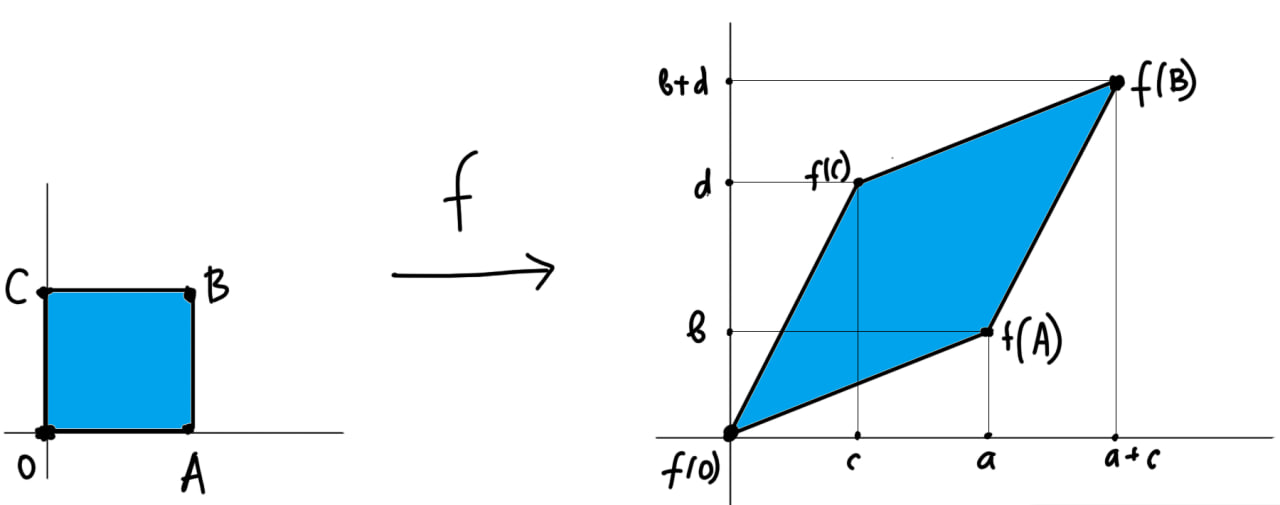
\includegraphics[scale = 0.5]{images/linear_map.jpg}
    \caption{Линейное отображение $f:\mathbb{R}^2 \to \mathbb{R}^2$, которое задаётся матрицей $A = \begin{pmatrix}
        a & c \\
        b & d
    \end{pmatrix}.$}
    \label{linear_map}
\end{figure}

Разумеется, не все отображения линейны. Однако некоторые из них \textit{локально} очень похожи на линейные. Чтобы формализовать эту идею, вводят понятие дифференцируемости.


\begin{definition}\label{diff_of_map(function)}
    Пусть $\mathbb{R}^n$, $\mathbb{R}^m$ -- векторные пространства с евклидовой нормой $\|\cdot \|$, $\mathscr{U} \subseteq \mathbb{R}^n$ -- открытое подмножество. Говорят, что отображение $F: \mathscr{U} \to \mathbb{R}^m$ \textit{дифференцируемо} в точке $\m{v} \in \mathbb{R}^n$, если существует зависящее от точки $\m{v}$ такое линейное отображение $\mathrm{d}F_{\mathbb{v}}:\mathbb{R}^n \to \mathbb{R}^m$, что
    \[
     F(\m{v} + \m{h})  = F(\m{v}) + \mathrm{d}F_\m{v}(\m{h}) + o(\|\m{h}\|),
    \]
где $o(\|\m{h}\|)$ -- вектор, норма которого при $\m{h} \to \m{0}$ бесконечно мала по сравнению с нормой $\|\m{h}\|$.

Другими словами, 
\[
     F(\m{v} + \m{h})  = F(\m{v}) + \mathrm{d}F_\m{v}(\m{h}) + \omega(\m{h}),
    \]
    где 
    \[
     \lim_{\m{h} \to \m{0}} \frac{\| \omega(\m{h})\|}{\| \m{h} \|} = 0.
    \]
Если отображение дифференцируемо в каждой точке $\mathscr{U}$, то говорят, что оно дифференцируемо на $\mathscr{U}$.

Линейное отображение $\mathrm{d}F_\m{v}$ называется \textit{дифференциалом отображения} в точке $\mathbb{v}$. 
\end{definition}

Прежде всего, мы должны убедиться, что линейные отображения тоже дифференцируемы.

\begin{lemma}
    Любое линейное отображение $\mathscr{L}: \mathbb{R}^n \to \mathbb{R}^m$ дифференцируемо
\end{lemma}
\begin{proof}
    Действительно, так как $\mathscr{L}$ -- линейное, то для любых $\m{x,h} \in \mathbb{R}^n$,
    \[
     \mathscr{L}(\m{x}+\m{h}) = \mathscr{L}(\m{x}) + \mathscr{L}(\m{h}),
    \]
    полагая теперь, что $\mathrm{d}\mathscr{L}_\mathbf{x}:=\mathscr{L}$, и так как нулевая функция $0$, очевидно, лежит в $o(||\m{h}||)$, мы и получаем требуемое.
\end{proof}

В дальнейшем нам понадобится следующая 
\begin{lemma}\label{||h||->0}
    Если $||\m{h}|| \to 0$, то все $h_i \to 0$, где $\m{h} = (h_1, \ldots, h_n) \in \mathbb{R}^n$.
\end{lemma}
\begin{proof}
    Так как $|| \m{h} || = \sqrt{h_1^2 + \cdots + h^2_n}$, то согласно неравенству (\ref{m<d<M}),
   \[
    \max_{1\le k \le n} |h_k| \le || \m{h} || \le \sqrt{n} \max_{1\le k \le n} |h_k|
   \] 
   поэтому если $||\m{h} || \to 0$, то $|h_k| \to 0$, что и доказывает требуемое.
\end{proof}


\begin{theorem}\label{diff=>contin}
    Если отображение $F: \mathbb{R}^n \to \mathbb{R}^m$ -- дифференцируемо в точке $\m{x}_0$, то оно непрерывно в этой точке.
\end{theorem}
\begin{proof}
Возьмём произвольный ненулевой вектор $\m{h} \in \mathbb{R}^n$ и рассмотрим выражение $F(\m{x}_0 + \m{h}) - F(\m{x}_0)$, так как $F$ -- дифференцируемо в $\m{x}_0$, то

\[
 \lim_{\m{h} \to \m{0}} \frac{F(\m{x}_0 + \m{h}) -  F(\m{x_0})}{|| \m{h} ||} = (\mathrm{d}F)_{\m{x}_0}(\m{h}) \in \mathbb{R}^m,
\]
тогда
\begin{eqnarray*}
    \lim_{\m{h} \to \m{0}}(   F(\m{x}_0 + \m{h}) - F(\m{x}_0)  ) &=& \lim_{\m{h} \to \m{0}} \frac{F(\m{x}_0 + \m{h}) -  F(\m{x_0})}{|| \m{h} ||} || \m{h}|| \\
    &=& (\mathrm{d}F)_{\m{x}_0}(\m{h}) \lim_{\m{h} \to \m{0}} || \m{h} || \\
    &=& 0,
\end{eqnarray*}
но тогда $\lim_{\m{v} \to \m{x}_0}F(\m{v}) = F(\m{x}_0)$ но это и означает непрерывность $F.$ \footnote{мы тут положили что $\m{v}: = \m{x}_0 +\m{h}$, а также что матрица }

\end{proof}


\section{Частные производные и матрица Якоби}

Рассмотрим теперь функцию $f:\mathbb{R}^n \to \mathbb{R}$, дифференцируемую на каком-то открытом $\mathscr{U} \subseteq \mathbb{R}^n$ или в фиксированной точке $\m{x}$. Тогда её дифференциал $(\mathrm{d}f)_\m{x}$ в точке $\m{x}$ задаётся матрицей размера $n\times 1$, $(\mathrm{d}f)_\m{x} = \begin{pmatrix}
    a_1 & \ldots & a_n
\end{pmatrix}$, где все $a_i$ есть функции от $\m{x}$. Наша цель -- найти эти $a_i$. Пусть $\m{h} = (h_1, \ldots, h_n)^\top \in \mathbb{R}^n$, тогда получаем
\begin{eqnarray*}
    f(\m{x} + \m{h}) - f(\m{x}) &=& (\mathrm{d}f)_\m{x}(\m{h}) + o(||\m{h}||) \\
    &=& \begin{pmatrix}
        a_1 & \ldots & a_n
    \end{pmatrix} \begin{pmatrix}
        h_1 \\ \vdots \\ h_n  \end{pmatrix} + o(||\m{h}||) \\
        &=& a_1h_1 + \cdots + a_nh_n + o(||\m{h}||).
\end{eqnarray*}

Видно, что $a_i$ не зависит от координат вектора $\m{h}$ кроме $h_i$ \ie чтобы найти $a_i$, нам достаточно рассмотреть вектор $\m{h}_i = h_i \m{e}_i$, где $\m{e}_i$ -- базисный вектор. В таком случае, $||\m{h}_i|| = |h_i|$ и тогда для каждого $1 \le i \le n$ мы получаем
\[
 f(\m{x} + h_i \m{e}_i) - f(\m{x}) = a_ih_i + o(|h_i|),
\]
таким образом, 
\[
 a_i = \lim_{h_i \to 0} \frac{f(\m{x} + h_i \m{e}_i) - f(\m{x})}{h_i},
\]
такое выражение называется \textit{частной производной функции по переменной $x_i$} и обозначается либо как $\frac{\partial f}{\partial x_i}$, либо как $f'_{x_i}$, \ie 
\begin{equation}\label{partial_i}
  \boxed{
 \frac{\partial f}{\partial x_i}: = \lim_{h_i \to 0} \frac{f(\m{x} + h_i \m{e}_i) - f(\m{x})}{h_i}}    
\end{equation}
если же мы хотим знать её значение в точке $\m{x}_0$, то получаем
\begin{equation}\label{partial_i(o)}
    \boxed{
      \frac{\partial f}{\partial x_i}(\m{x}_0): = \lim_{h_i \to 0} \frac{f(\m{x}_0 + h_i \m{e}_i) - f(\m{x}_0)}{h_i}.
    }
\end{equation}

Таким образом, в случае функции $f:\mathbb{R}^n \to \mathbb{R}$ дифференциал в точке $\m{x}_0$ находится по формуле
\[
 (\mathrm{d}f)_{\m{x}_0}: = \begin{pmatrix}
     \frac{\partial f}{\partial x_1}(\m{x}_0) & \ldots & \frac{\partial f}{\partial x_n}(\m{x}_0)
 \end{pmatrix}.
\]

Тогда для любого вектора $\m{h} = (h_1,\ldots, h_n)^\top$,
\[
 (\mathrm{d}f)_{\m{x}_0}(\m{h}) =  \begin{pmatrix}
     \frac{\partial f}{\partial x_1}(\m{x}_0) & \ldots & \frac{\partial f}{\partial x_n}(\m{x}_0)
 \end{pmatrix} \begin{pmatrix}
     h_1 \\ \vdots \\ h_n
 \end{pmatrix} = ((\mathrm{d}f)_{\m{x}_0}, \m{h}),
\]
где последняя скобка означает скалярное произведение.

\begin{definition}
    Дифференциал $(\mathrm{d}f)_{\m{x}_0}$ функции $f: \mathbb{R}^n \to \mathbb{R}$ в точке $\m{x}_0$ называется \textit{градиентом} функции. Принято обозначение $\nabla_{\m{x}_0}f$ для градиента.
\end{definition}

\begin{mydanger}{\bf{!}}
 Мы видим, что дифференциал функции $f:\mathbb{R}^n \to \mathbb{R}$ похож на вектор, но вовсе не есть вектор, так как он определён на векторах и принимает от них числовые значения. Другими словами, это элемент двойственного векторного пространства $V^*: = \mathrm{Hom}(V, \mathbb{R})$ к векторному пространству $V$. Элементы из $V^*$ называются \textit{функционалами} или \textit{ковекторами}.    
\end{mydanger}


Рассмотрим теперь отображение $F: \mathbb{R}^n \to \mathbb{R}^m$, которое задаётся следующим образом:
\[
 F: \begin{pmatrix}
      x_1 \\ \vdots \\ x_n
 \end{pmatrix} \mapsto 
 \begin{pmatrix}
     f_1(x_1, \ldots, x_n) \\ \vdots \\ f_m(x_1, \ldots, x_n),
 \end{pmatrix}
\]
где $f_i:\mathbb{R}^n \to \mathbb{R}$. Потребуем, чтобы $F$ была дифференцируема в каком-то открытом $\mathscr{U} \subseteq \mathbb{R}^n$ или в фиксированной точке $\m{x}_0$. 

Тогда 
\[
 F(\m{x} + \m{h}) - F(\m{h}) = (\mathrm{d}_\m{x}F)(\m{h}) + o(||\m{h}||).
\]

Пусть $\m{h} = h_i \m{e}_i$, тогда $(\mathrm{d}_\m{x}F)(\m{e}_i)$ есть $i$-ый столбец матрицы $(\mathrm{d}_\m{x}F)(\m{h})$, и мы получаем равенство
\[
 \begin{pmatrix}
     f_1(x_1, \ldots, x_i + h_i, \ldots, x_n) -f_1(x_1, \ldots, x_i, \ldots, x_n) \\
     \vdots \\
     f_m(x_1, \ldots, x_i + h_i, \ldots, x_n) -f_m(x_1, \ldots, x_i, \ldots, x_n)
 \end{pmatrix} = h_i(\mathrm{d}_\m{x}F)(\m{e}_i) + o(|h_i|), \qquad 1 \le i \le n
\]
тогда
\[
 (\m{d}F)_\m{x}(\m{e}_i) = \begin{pmatrix}
     \frac{\partial f_1}{\partial x_i} \\ \vdots \\ \frac{\partial f_m}{\partial x_i}
 \end{pmatrix}
\]
и в итоге
\[
 (\m{d}F)_\m{x} = \begin{pmatrix}
     \frac{\partial f_1}{\partial x_1} & \ldots & \frac{\partial f_1}{\partial x_n} \\
     \vdots & \ddots & \vdots \\
     \frac{\partial f_m}{\partial x_1} & \ldots & \frac{\partial f_m}{\partial x_n}
 \end{pmatrix}, \qquad 
 (\m{d}F)_{\m{x}_0} = \begin{pmatrix}
     \frac{\partial f_1}{\partial x_1}({\m{x}_0}) & \ldots & \frac{\partial f_1}{\partial x_n} ({\m{x}_0}) \\
     \vdots & \ddots & \vdots \\
     \frac{\partial f_m}{\partial x_1} ({\m{x}_0}) & \ldots & \frac{\partial f_m}{\partial x_n} ({\m{x}_0})
     \end{pmatrix}
    \]

Такая матрица называется \textit{матрицей Якоби} отображения $F.$


\section{Касательная плоскость и её базис}

Итак, мы уже поняли, что если $f:\mathbb{R} \to \mathbb{R}$ -- дифференцируемая функция в точке $x_0$, то значение её производной в точке $x_0$ можно понимать как наклон касательной к графику этой функции в точке $(x_0, f(x_0))$. Пусть теперь $f:\mathbb{R}^n \to \mathbb{R}$ -- функция от $n>1$ переменных, и пусть она дифференцируема в точке $\m{x}_0$. Тогда возникает вопрос, о чём говорят значения её частных производных в точке $\m{x}_0$?

Для наглядности мы ограничимся случаем, когда $n=2$, случай, когда $n >2$, совершенно аналогичен.

Итак, пусть у нас есть функция $f:\mathbb{R}^2 \to \mathbb{R}$, которая дифференцируема в точке $(x_0,y_0)$. Рассечём её график плоскостью, параллельной плоскости $yz$, через точку $(x_0,y_0,0)$. Тогда мы получаем кривую, которая представляется какой-то функцией от $y$. Тогда, согласно определению частой производной, мы видим, что наклон к графику этой функции и есть значение $\frac{\partial f}{\partial y}(x_0,y_0)$.

\begin{figure}[h!]
    \centering
    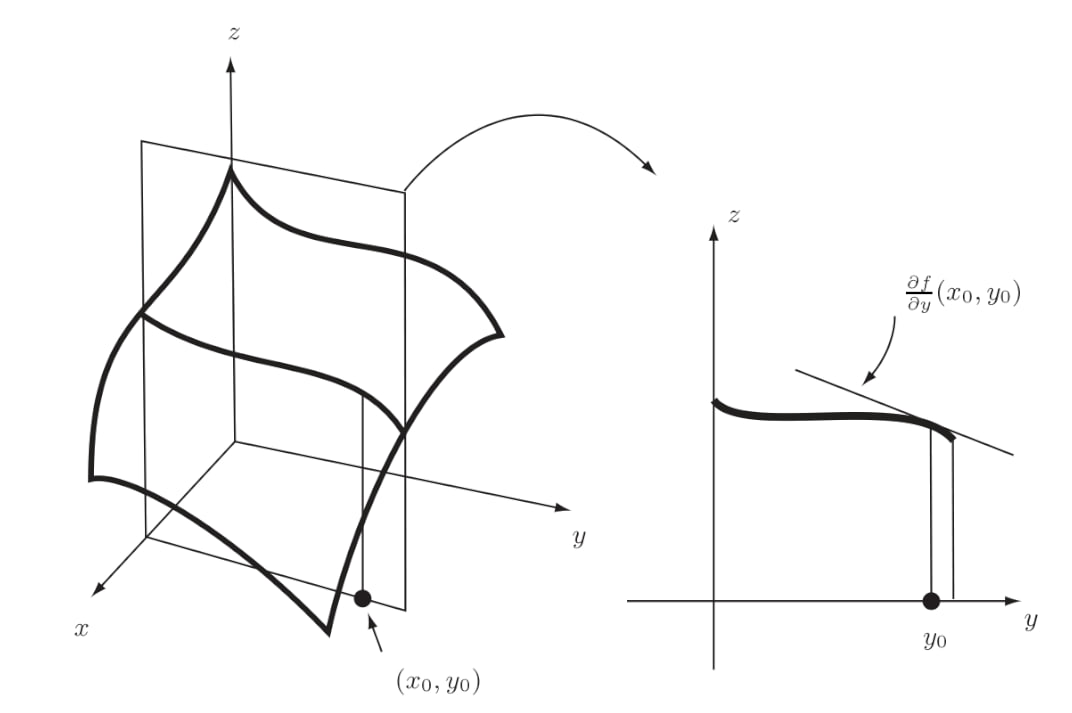
\includegraphics[scale = 0.6]{images/partial_deri.jpg}
    \caption{Мы рассекли график $z =f(x,y)$ плоскостью, параллельной плоскости $yz$, через точку $(x_0,y_0,0)$. Тогда мы получаем кривую, которая представляется какой-то функцией от $y$, и её наклон и есть $\frac{\partial f}{\partial y}(x_0,y_0)$.}
    \label{fig:enter-label}
\end{figure}

\subsection{Построение касательной плоскости}

С другой стороны, мы можем пойти дальше и рассечь этот же график, но уже не параллельной ни плоскости $yz$, ни плоскости $xz$. Как тогда вычислить наклон?

Чтобы ответить на этот вопрос, мы рассмотрим множество всех прямых, которые касаются графика в точке $(x_0, y_0, f(x_0,y_0))$. Такое множество мы называем \textit{касательной плоскостью} к графику $z = f(x,y).$

Уравнение плоскости, которая проходит через точку $(0,0,0)$, имеет вид $z = Ax + By$. Тогда сдвинув эту плоскость к точке $(x_0, y_0, f(x_0,y_0))$, мы получим тогда такое уравнение плоскости: $z - f(x_0,y_0) = A(x-x_0) + B(y-y_0)$. Осталось найти коэффициенты $A,B$, чтобы эта плоскость стала касательной. Пересечём эту плоскость с плоскостью $y=y_0$, в результате мы получаем прямую $z(x, y_0) - f(x_0,y_0) = A(x-x_0)$, тогда потребовав, чтобы эта прямая была касательной, мы получаем, что $A = \frac{\partial f}{\partial x}(x_0,y_0)$. Аналогично находим $B = \frac{\partial f}{\partial y}(x_0,y_0)$.

Итак, мы получаем следующее определение
\begin{definition}
 Пусть задана поверхность $M$ уравнением $z  = f(x,y)$, рассмотрим точку $P=(x_0,y_0,z_0)$ на поверхности $M$. Пусть существуют частные производные $\frac{\partial f}{\partial x}(x_0,y_0)$, $\frac{\partial f}{\partial y}(x_0,y_0)$. Тогда множество точек удовлетворяющих уравнению 
 \[
z - f(x_0,y_0) = \left.\frac{\partial f}{\partial x}\right|_{(x_0,y_0)} (x-x_0) + \left.\frac{\partial f}{\partial y}\right|_{(x_0,y_0)} (y-y_0)
\]
называется \textit{касательной плоскостью} к поверхности $M$ в точке $P$, и обозначается так $T_PM$.
\end{definition}



\subsection{Базис касательной плоскости}
Нам удобно принять слудующие обозначения. Пусть $P = (x_0,y_0,z_0)$ принадлежит поверхности $M : =\{(x,y,z)\, : \, z  = f(x,y) \} $, тогда $z_0 = f(x_0,y_0)$. Пусть $p: = (x_0,y_0)$, тогда $P = (p, f(p))$.

Следующая теорема описывает касательную плоскость в теримнах базиса.

\begin{theorem}
 Касательная плоскость $T_PM$ к поверхности $M: = \{(x,y,z)\, : \, z  = f(x,y) \}$ в точке $P= (x_0,y_0,z_0)$, как векторное пространство может быть представлено в виде
 \[
 T_PM \cong \mathrm{Span}_\mathbb{R}(\m{v}_x, \m{v}_y),
 \]
 где
 \[
  \m{v}_x : = \bigl( 1,0, f'_x(p) \bigr)^\top, \qquad  \m{v}_y : = \bigl( 0,1, f'_y(p) \bigr)^\top
\]
и более того эти векторы образуют базис $T_PM.$
\end{theorem}
\begin{proof}
 
Сохраним прежние обозначения и рассмотрим теперь произвольную точку $P_1(x_1,y_1,z_1)$, возникаем вектор $\m{h}: = (x_1 - x_0, y_1-y_0, z_1-z_0)^\top$. Мы хотим понять, когда этот вектор будет лежать в касательной плоскости $T_PM.$ Для краткости, мы примем обозначения $h_1: = x_1 - x_0,$, $h_2: = y_1- y_0$, $h_3: = z_1 - z_0$, таким образом $\m{h} = (h_1,h_2,h_3)^\top$.

Далее, согласно определению касатальной плоскости, $\m{h} \in T_pM$ тогда и только тогда, когда 
 \[
z_1 - f(x_0,y_0) = f_x'(p) (x_1-x_0) + f'_y(p) (y_1-y_0)
\]
или в новых обозначениях
\[
 h_3 = f_x'(p) \cdot h_1 + f'_y(p) \cdot h_2.
\]

Таким образом, имеем
\[
 \m{h} = \begin{pmatrix}
     h_1 \\ h_2 \\h_3
 \end{pmatrix} = \begin{pmatrix}
     h_1 \\ h_2 \\ f_x'(p) \cdot h_1 + f'_y(p) \cdot h_2
 \end{pmatrix} = \begin{pmatrix}
     h_1 \\ 0 \\ f_x'(p) \cdot h_1
 \end{pmatrix} + \begin{pmatrix}
     0 \\ h_2 \\ f'_y(p) \cdot h_2
 \end{pmatrix} = h_1 \begin{pmatrix}
     1 \\ 0 \\ f'_x(p)
 \end{pmatrix} + h_2 \begin{pmatrix}
     0 \\ 1 \\ f'_y(p)
 \end{pmatrix}
\]
что и означает,
 \[
 T_PM \cong \mathrm{Span}_\mathbb{R}(\m{v}_x, \m{v}_y),
 \]
 где
 \[
  \m{v}_x : = \bigl( 1,0, f'_x(p) \bigr)^\top, \qquad  \m{v}_y : = \bigl( 0,1, f'_y(p) \bigr)^\top.
\]

Допустим что имеются такие числа $\alpha, \beta$, что $\alpha \cdot\m{v}_x+ \beta \cdot \m{v}_y = \m{0}$.

Имеем
\[
 \alpha \cdot\m{v}_x+ \beta \cdot \m{v}_y =  \alpha \begin{pmatrix}
     1 \\ 0 \\ f'_x(p)
 \end{pmatrix} + \beta \begin{pmatrix}
     0 \\ 1 \\ f'_y(p) \end{pmatrix} = \begin{pmatrix}
        \alpha \\ \beta \\ \alpha \cdot f_x'(p) + \beta \cdot f'_y(p)
     \end{pmatrix} = \begin{pmatrix}
         0\\0\\0
     \end{pmatrix}
\]
откуда $\alpha = \beta = 0$, \textit{т.е.,} векторы $\m{v}_x$, $\m{v}_y$ линейно неависимы. Это завершаешт доказательство.
\end{proof}


\section{Производная по направлению}
Вернёмся ещё раз к предыдущему рисунку. Введём обозначения. Пусть $P$ -- вертикальная плоскость, проходящая через точку $(x_0,y_0)$. Пусть $\ell$ -- прямая, по которой $P$ пересекает плоскость $xy$. Касательную прямую к кривой, которую высекает плоскость $P$, мы обозначим через $L$. Касательная плоскость в точке $(x_0,y_0, f(x_0,y_0))$ пусть будет $T$. Далее, рассмотрим вектор $\m{v}$, который лежит на $\ell$, выходит из точки $(x_0,y_0)$ и кончается в $(x_0+a, y_0 +b)$, \ie имеет координаты $(a,b)$.

\begin{figure}[h!]
    \centering
    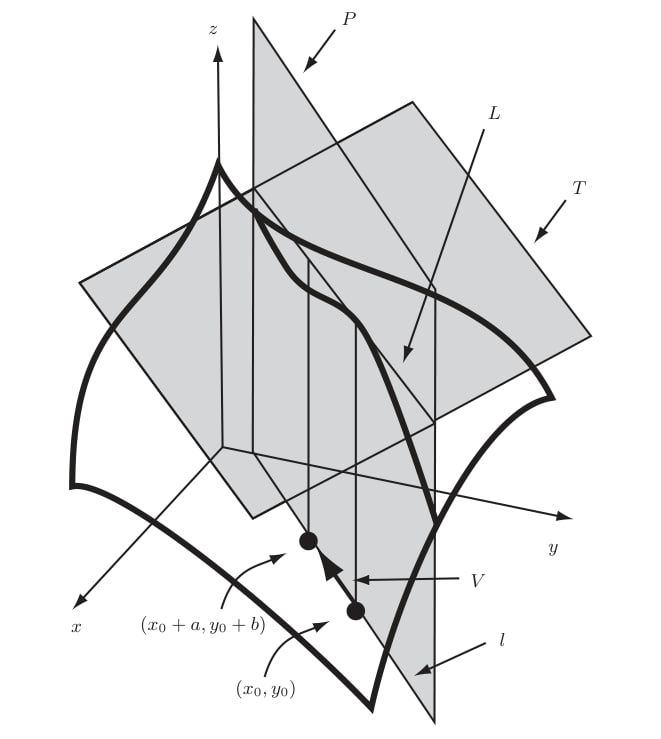
\includegraphics[scale =0.7]{images/direction_der2.jpg}
    \caption{Caption}
    \label{fig:enter-label}
\end{figure}



Имеем
\begin{eqnarray*}
    T(x_0 + a, y_0 + b) - T(x_0,y_0) &=& \left.\frac{\partial f}{\partial x}\right|_{(x_0,y_0)} (x_0 +a-x_0) + \left.\frac{\partial f}{\partial y}\right|_{(x_0,y_0)} (y_0 +b-y_0) \\
    &=& a\left.\frac{\partial f}{\partial x}\right|_{(x_0,y_0)} + b\left.\frac{\partial f}{\partial y}\right|_{(x_0,y_0)} \\
    &=& \langle \m{v} , \nabla f (x_0, y_0) \rangle
\end{eqnarray*}




Тогда, чтобы вычислить наклон, нужно потребовать, чтобы один из катетов в прямоугольном треугольнике был равен $1$, таким образом, если $a^2 + b^2 = 1$, то искомый наклон и есть число $\langle \m{v} , \nabla f (x_0, y_0) \rangle.$

Итак мы получаем следующее
\begin{definition}
    Пусть дана точка $\m{p} \in \mathbb{R}^n$, вектор $\m{v}\in \mathbb{R}^n$ и пусть $f:\mathbb{R}^n \to \mathbb{R}$ -- функция. Тогда \textit{производная по направлению $\m{v}$ вычисленная в точке $\m{p}$} есть выражение вида
    \[
     (\nabla_\m{v}f)(\m{p}): = \frac{1}{\| \m{v}\|} (\mathrm{d}f)_\m{p} \m{v},
    \]
\end{definition}
где справа стоит умножение матриц. А именно, так как
\[
 (\mathrm{d}f)_\m{p} = \begin{pmatrix}
     f'_{x_1}(\m{p}) & \ldots & f'_{x_n}(\m{p})
 \end{pmatrix} \in \mathrm{Mat}_{1\times n}(\mathbb{R}),
\]
то получаем
\[
 \boxed{
 (\nabla_\m{v}f)(\m{p}) =\frac{1}{\|\m{v}\|} \left(  f'_{x_1}(\m{p})v_1 + \cdots + f'_{x_n}(\m{p}) v_n\right).
 }
\]

\section{Необходимые и достаточные условия дифференцируемости}

\subsection{Необходимые условия}

Что касается необходимых условия дифференцируемости, то мы их уже знаем. Но для удобства мы сделаем из этого следующую теорему:



\begin{theorem}
    Если функция $f:\mathbb{R}^n \to \mathbb{R}$ дифференцируема на каком-то открытом $\mathscr{U} \subseteq \mathbb{R}^n$ или в фиксированной точке $\m{x}$, то она имеет в этой точке частные производные по всем переменным.
\end{theorem}

\begin{proof}
   Пусть $f:\mathbb{R}^n \to \mathbb{R}$, дифференцируемая на каком-то открытом $\mathscr{U} \subseteq \mathbb{R}^n$ или в фиксированной точке $\m{x}$. Тогда её дифференциал $(\mathrm{d}f)_\m{x}$ в точке $\m{x}$ задаётся матрицей размера $n\times 1$, $(\mathrm{d}f)_\m{x} = \begin{pmatrix}
    a_1 & \ldots & a_n
\end{pmatrix}$, где все $a_i$ есть функции от $\m{x}$. Наша цель -- найти эти $a_i$. Пусть $\m{h} = (h_1, \ldots, h_n)^\top \in \mathscr{U} \subseteq \mathbb{R}^n$, тогда получаем
\begin{eqnarray*}
    f(\m{x} + \m{h}) - f(\m{x}) &=& (\mathrm{d}f)_\m{x}(\m{h}) + o(||\m{h}||) \\
    &=& \begin{pmatrix}
        a_1 & \ldots & a_n
    \end{pmatrix} \begin{pmatrix}
        h_1 \\ \vdots \\ h_n  \end{pmatrix} + o(||\m{h}||) \\
        &=& a_1h_1 + \cdots + a_nh_n + o(||\m{h}||).
\end{eqnarray*}

Видно, что $a_i$ не зависит от координат вектора $\m{h}$ кроме $h_i$ \ie чтобы найти $a_i$, нам достаточно рассмотреть вектор $\m{h}_i = h_i \m{e}_i$, где $\m{e}_i$ -- базисный вектор. В таком случае, $||\m{h}_i|| = |h_i|$, и тогда для каждого $1 \le i \le n$ мы получаем
\[
 f(\m{x} + h_i \m{e}_i) - f(\m{x}) = a_ih_i + o(|h_i|),
\]
таким образом, 
\[
 a_i = \lim_{h_i \to 0} \frac{f(\m{x} + h_i \m{e}_i) - f(\m{x})}{h_i},
\]
такое выражение называется \textit{частной производной функции по переменной $x_i$} и обозначается либо как $\frac{\partial f}{\partial x_i}$, либо как $f'_{x_i}$, \ie 
\[
 \frac{\partial f}{\partial x_i}: = \lim_{h_i \to 0} \frac{f(\m{x} + h_i \m{e}_i) - f(\m{x})}{h_i},
\]
если же мы хотим знать её значение в точке $\m{x}_0$, то получаем
\[
 \frac{\partial f}{\partial x_i}(\m{x}_0): = \lim_{h_i \to 0} \frac{f(\m{x}_0 + h_i \m{e}_i) - f(\m{x}_0)}{h_i}.
\]
\end{proof}


Таким образом, в случае функции $f:\mathbb{R}^n \to \mathbb{R}$, дифференциал в точке $\m{x}_0$ находится по формуле
\[
 (\mathrm{d}f)_{\m{x}_0}: = \begin{pmatrix}
     \frac{\partial f}{\partial x_1}(\m{x}_0) & \ldots & \frac{\partial f}{\partial x_n}(\m{x}_0)
 \end{pmatrix}.
\]

\subsection{Достаточные условия дифференцируемости}

\begin{theorem}
Если все частные производные \( \frac{\partial f}{\partial x_i} \) существуют в окрестности \( \mathbf{a} \) и непрерывны в \( \mathbf{a} \), то \( f \) дифференцируема в \( \mathbf{a} \).    
\end{theorem}


\begin{proof} Для простоты мы начнём со случая двух переменных.

Итак, пусть функция \( f: \mathbb{R}^2 \to \mathbb{R} \) имеет непрерывные частные производные \( \frac{\partial f}{\partial x} \) и \( \frac{\partial f}{\partial y} \) в окрестности $\mathscr{U}$ точки \( \mathbf{a} = (x_0, y_0) \). Покажем что \( f \) дифференцируема в точке \( \mathbf{a} \).

\begin{figure}[h!]
    \centering
     \begin{tikzpicture}[>=Stealth, scale=1.2]
    % Координатные оси
    \draw[->] (-1,0) -- (6,0) node[below] {$x$};
    \draw[->] (0,-1) -- (0,5) node[left] {$y$};
    
    % Область U (светло-серый круг)
    \fill[lightgray!30] (3.5,2.5) circle (2cm);
    \node at (3,4) {$\mathscr{U}$};
    
    % Координатные линии и подписи для точки a+h
    \draw[dashed] (5,0) -- (5,3) -- (0,3);
    \filldraw (5,3) circle (1.5pt) node[above right] {$\mathbf{a} + \mathbf{h}$};
    
    % Вектор h и отрезки
    \draw[blue, thick] (3,2) -- node[midway, below] {$I_1$} (5,2);
    \draw[red, thick] (5,2) -- node[midway, right]  {$I_2$} (5,3);
    
    % Подпись вектора h
    %\node at (4.5,1.5) {$\mathbf{h} = (h_1, h_2)$};
    
    % Деления на осях
    \foreach \x in {1,...,5}
        \draw (\x,0.1) -- (\x,-0.1) node[below] {};
    \foreach \y in {1,...,4}
        \draw (0.1,\y) -- (-0.1,\y) node[left] {};
        
    %подписи координат
    \draw(3,0) node [below]{$x_0$};
    \draw(5,0) node [below]{$x_0+h_1$};
    \draw(0,2) node [left]{$y_0$};
    \draw(0,3) node [left]{$y_0+h_2$};

     % Координатные линии и подписи для точки a
    \draw[dashed] (3,0) -- (3,2) -- (0,2);
    \filldraw (3,2) circle (1.5pt) node[below left] {$\mathbf{a}$};    
\end{tikzpicture}
    \caption{В окрестности $\mathscr{U}$ точки $\m{a}$ мы имеем два отрезка, ограничения на которых мы получаем функции от одной координаты.}
    \label{fig:enter-label}
\end{figure}

Возьмём вектор \( \mathbf{h} = (h_1, h_2) \) такой, что $\m{a+h} \in \mathscr{U}$, тогда получаем два отрезка
\[
 I_1: = [ (x_0,y_0), (x_0 + h_1, y_0) ], \qquad I_2: = [ (x_0+h_1,y_0), (x_0+h_1, y_0+h_2) ],
\]
которые лежат в $\mathscr{U}$. Согласно условию, и определению частных производных, функции\footnote{это уже функции от одной переменной} $f_1: = f|_{I_1}$, $f_2: = f|_{I_2}$ дифференцируемы на отрезках $I_1, I_2$.

Тогда, согласно теореме Лагранжа \ref{Langrange}, существуют числа \( \theta_1, \theta_2 \in (0,1) \) такие, что
\begin{eqnarray*}
    f_1(x_0 + h_1, y_0) - f_1(x_0, y_0) &=& f'_1(x_0+\theta_1h_1, y_0)h_1,\\
    f_2(x_0 +h_1, y_0+h_2) - f_2(x_0+h_1, y_0) &=& f'_2(x_0 + h_1, y_0+\theta_2h_2)h_2.
\end{eqnarray*}

Согласно определению частных производных, это можно записать так

\begin{eqnarray*}
    f_1(x_0 + h_1, y_0) - f_1(x_0, y_0) &=& f'_x(x_0+\theta_1h_1, y_0)h_1,\\
    f_2(x_0 +h_1, y_0+h_2) - f_2(x_0+h_1, y_0) &=& f'_y(x_0 + h_1, y_0+\theta_2h_2)h_2.
\end{eqnarray*}

Тогда имеем

\begin{eqnarray*}
     f(\mathbf{a} + \mathbf{h}) - f(\mathbf{a}) &=& f(x_0 + h_1, y_0 + h_2) - f(x_0, y_0) \\
     &=& \Bigl( f(x_0 + h_1, y_0 + h_2) - f(x_0 + h_1, y_0) \Bigr)  + \Bigl(f(x_0 + h_1, y_0) - f(x_0, y_0)\Bigr)\\
     &=&f'_y(x_0 + h_1, y_0+\theta_2h_2)h_2 + f'_x(x_0+\theta_1h_1, y_0)h_1. 
\end{eqnarray*}

В более удобном виде это можно записать так
\[
 f(\mathbf{a} + \mathbf{h}) - f(\mathbf{a}) = f'_x(\m{a} + \theta_1 h_1 \m{e}_1)h_1 + f_y'(\m{a} + h_1\m{e}_1 + \theta_2 h_2 \m{e}_2)h_2.
\]

Имеем
\begin{eqnarray*}
    f(\mathbf{a} + \mathbf{h}) - f(\mathbf{a}) &=& f'_x(\m{a} + \theta_1 h_1 \m{e}_1)h_1 + f_y'(\m{a} + h_1\m{e}_1 + \theta_2 h_2 \m{e}_2)h_2 \\
    && + \Bigl( f'_x(\m{a})h_1 + f_y'(\m{a})h_2 \Bigr) - \Bigl(f'_x(\m{a})h_1 + f_y'(\m{a})h_2 \Bigr)
\end{eqnarray*}

Запишем это выражение следующим образом

\[
    f(\mathbf{a} + \mathbf{h}) - f(\mathbf{a}) = \underbrace{f'_x(\mathbf{a})h_1 + f'_y(\mathbf{a})h_2}_{\mathrm{d}f_\m{a}(\mathbf{h})} + R(\mathbf{h})
    \]
где
  \[
  R(\mathbf{h}) := \Bigl(f_x'(\m{a}+ \theta_1 h_1) - f_x'(\mathbf{a})\Bigr)h_1 + \Bigl(f_y'(\m{a} + h_1\m{e}_1 + \theta_2 h_2 \m{e}_2) - f'_y(\mathbf{a})\Bigr)h_2.
 \]

Покажем, что $R(\m{h}) = o(\|\m{h}\|)$, при $\m{h} \to \m{0}$. Действительно, так как $|h_i| \le \max \{ |h_1|,\ldots, |h|_n \}$, тогда, согласно неравенству Леммы \ref{m<d<M},
\[
\max_{1 \le k \le n} |h_k| \le \sqrt{\sum_{k=1}^n h_k^2} \le \sqrt{n} \max_{1\le k \le n} |h_k|,
\]
получаем $\frac{h_i}{\|\m{h}\|} \le 1$. Тогда имеем

\begin{eqnarray*}
  \left| \frac{R(\mathbf{h})}{\|\mathbf{h}\|} \right| &=& \frac{1}{\|\m{h}\|} \left| \Bigl(f_x'(\m{a}+ \theta_1 h_1) - f_x'(\mathbf{a})\Bigr)h_1 + \Bigl(f_y'(\m{a} + h_1\m{e}_1 + \theta_2 h_2 \m{e}_2) - f'_y(\mathbf{a})\Bigr)h_2 \right| \\
  &\leq& \frac{|h_1|}{\|\mathbf{h}\|}  \cdot \left|f_x'(\m{a}+ \theta_1 h_1) - f_x'(\mathbf{a}) \right|  + \frac{|h_2|}{\|\mathbf{h}\|}  \cdot \left|f_y'(\m{a} + h_1\m{e}_1 + \theta_2 h_2 \m{e}_2) - f'_y(\mathbf{a}) \right|  \\
  &\le & \left| \Bigl(f_x'(\m{a}+ \theta_1 h_1) - f_x'(\mathbf{a})\Bigr) \right|  +  \left|f_y'(\m{a} + h_1\m{e}_1 + \theta_2 h_2 \m{e}_2) - f'_y(\mathbf{a}) \right|
\end{eqnarray*}

Так как при $\m{h} \to \m{0}$, имеем $h_1,h_2 \to 0$, то в силу непрерывности частных производных имеем
\[
 \lim_{h_1,h_2 \to 0} \left|  f_x'(\m{a}+ \theta_1 h_1) - f_x'(\mathbf{a}) \right| =0,  \qquad \lim_{h_1,h_2 \to 0} \left|f_y'(\m{a} + h_1\m{e}_1 + \theta_2 h_2 \m{e}_2) - f'_y(\mathbf{a}) \right| = 0
\]
\textit{т.е.,} $R(\m{h}) = o(\|\m{h}\|)$, при $\m{h} \to \m{0}$. Это завершает доказательство в случае двух переменных.

В общем случае, мы тогда можем аналогично рассмотреть отрезки 


\[
    f(\mathbf{a} + \mathbf{h}) - f(\mathbf{a}) = \sum_{i=1}^n \left[ f(\mathbf{a} + \mathbf{h}^{(i)}) - f(\mathbf{a} + \mathbf{h}^{(i-1)}) \right],
    \]
    где \( \mathbf{h}^{(i)} = (h_1, \dots, h_i, 0, \dots, 0) \).

    \item Применяем теорему Лагранжа:
    \[
    f(\mathbf{a} + \mathbf{h}^{(i)}) - f(\mathbf{a} + \mathbf{h}^{(i-1)}) = h_i \frac{\partial f}{\partial x_i}(\mathbf{a} + \mathbf{c}_i),
    \]
    где \( \mathbf{c}_i: = \m{h}^{(i-1)} + \theta_ih_i \m{e}_i \) — точка на соответствующем отрезке.

    \item Линейная часть и остаток:
    \[
    f(\mathbf{a} + \mathbf{h}) - f(\mathbf{a}) = \nabla f(\mathbf{a}) \cdot \mathbf{h} + \underbrace{\sum_{i=1}^n h_i \left( \frac{\partial f}{\partial x_i}(\mathbf{a} + \mathbf{c}_i) - \frac{\partial f}{\partial x_i}(\mathbf{a}) \right)}_{R(\mathbf{h})}.
    \]

    \item Оценка остатка:
    \[
    |R(\mathbf{h})| \leq \sum_{i=1}^n |h_i| \cdot \epsilon \leq \epsilon \|\mathbf{h}\|_1 = o(\|\mathbf{h}\|).
    \]
\end{proof}

\section{Дифференциал композиции}


\subsection{Непрерывность линейных отображений}

Напомним, что линейное отображение $L: \mathbb{R}^n \to \mathbb{R}^m$ -- это такое отображение, что
\[
 L(\alpha \m{v} + \beta \m{u}) = \alpha L(\m{v}) + \beta L(\m{u}),
\]
для любых $\m{v}, \m{u} \in \mathbb{R}^n$, $\alpha,\beta \in \mathbb{R}$.

Заметим, что 
\[
 L(\m{0}_n) = \m{0}_m,
\]
где $\m{0}_k$ -- нулевой вектор векторного пространства $\mathbb{R}^k$.


\begin{definition}
    Говорят, что линейное отображение $L: \mathbb{R}^n \to \mathbb{R}^m$ ограничено, если существует такое $K \ge 0$, что для любого $\m{v} \in \mathbb{R}^n$, $|| L(\m{v}) || \le K ||\m{v}||.$
\end{definition}

\begin{proposition}\label{contous_of_linear}
    Пусть $L: \mathbb{R}^n \to \mathbb{R}^m$ -- линейное отображение. Тогда следующие утверждения равносильны:
    \begin{enumerate}
        \item $L$ -- непрерывно.
        \item $L$ -- непрерывно в нуле.
        \item Существует такое $C > 0$, что $|| L(\m{v})| \le C ||\m{v}||$ для любого $\m{v} \in \mathbb{R}^n$
    \end{enumerate}
\end{proposition}
\begin{proof}
(1) $\Longrightarrow$ (2). Это просто следует из того, что если $L$ непрерывно, то оно непрерывно во всех точках $\mathbb{R}$, в частности и в нуле тоже.

(2) $\Longrightarrow$ (3). Если $L$ непрерывно в нуле, то это значит, что для любого $\varepsilon >0$ можно всегда найти такое $\delta>0$, что из $||\m{h}|| <\delta$ будет следовать $||L(\m{h})|| <\varepsilon$. Пусть $\varepsilon = 1$, тогда мы всегда найдём такой $\delta>0$, что если $|| \m{h} || < \delta$, то $|| L(\m{h})|| < 1$. Зафиксируем такое $\delta.$

Возьмём теперь произвольный ненулевой вектор\footnote{Аксиома Выбора позволяет.} $\m{v}$, тогда имеем
\begin{eqnarray*}
 || L(\m{v}) || &=& \left\| \frac{2}{\delta} || \m{v} || L\left(  \frac{\delta \m{v}}{2 || \m{v} ||}\right) \right\| \\
 &=&  \frac{2}{\delta} || \m{v}|| \cdot \left\| L\left(  \frac{\delta \m{v}}{2 || \m{v} ||}\right) \right\| < \frac{2}{\delta} || \m{v}||
\end{eqnarray*}
потому что 
\[
 \left\|\frac{\delta \m{v}}{2 || \m{v} ||} \right\| = \frac{\delta}{2} < \delta,
\]
и так как $\delta$ фиксировано, мы получаем требуемое.

(3) $\Longrightarrow$ (1). Имеем
\[
 || L(\m{v}) - L(\m{u}) || = || L(\m{v} - \m{u}) || \le K || \m{u} - \m{v} ||,
\]
тогда если $||\m{u} - \m{v}|| < \delta$, то $|| L(\m{v}) - L(\m{u}) ||< K \delta$,
поэтому для любого $\varepsilon >0$, если мы положим, что $0<\delta < \frac{\varepsilon}{K}$, то мы и получаем непрерывность $L$.
\end{proof}




\begin{lemma}\label{linear_is_contious}
    Любое линейное отображение $L: \mathbb{R}^n \to \mathbb{R}^m$ непрерывно. 
\end{lemma}
\begin{proof}
Пусть $L$ задаётся матрицей $(a_{i,j})_{1\le i \le n, 1 \le j \le m}$, тогда

\[
 L(\m{v}) = \begin{pmatrix}
     a_{11} & \ldots & a_{1n} \\
     \vdots & \ddots & \vdots \\
     a_{m1} & \ldots & a_{mn}
 \end{pmatrix}   \begin{pmatrix}
     v_1 \\ \vdots \\ v_n
 \end{pmatrix} = \begin{pmatrix}
     a_{11}v_1 + \cdots + a_{1n}v_n \\
     \vdots \\
     a_{m1}v_1 + \cdots + a_{mn}v_n 
 \end{pmatrix} = (u_1, \ldots, u_m)^\top =:\m{u} \in \mathbb{R}^m,
\] 
тогда
\begin{eqnarray*}
    ||L(\m{v})|| &=& ||\m{u}|| \\
    &=& \sqrt{(a_{11}v_1 + \cdots + a_{1n}v_n)^2 + \cdots + (a_{m1}v_1 + \cdots + a_{mn}v_n)^2} \\
    &\le & \sqrt{ m } \max_{1 \le k \le m} \left| a_{k1}v_1 + \cdots + a_{kn}v_n  \right| \\
    &\le & \sqrt{ m } \max_{1 \le k \le m} \left( |a_{k1}| \cdot |v_1| + \cdots + |a_{kn}| \cdot |v_n| \right) \\
    &\le & \sqrt{ m } \max_{1 \le k \le m} \left(|a_{k1}| \cdot || \m{v}|| + \cdots + |a_{kn}| \cdot || \m{v}||  \right) \\
    &=& \sqrt{ m } \max_{1 \le k \le m}\left(|a_{k1}|  + \cdots + |a_{kn}|   \right) \cdot || \m{v}|| \\
    &=& K || \m{v}||,
\end{eqnarray*}
где $K: = \sqrt{ m } \max_{1 \le k \le m}\left(|a_{k1}|  + \cdots + |a_{kn}|   \right)$, тогда по Предложению \ref{contous_of_linear} оно непрерывно. 
\end{proof}


\subsection{Дифференциал композиции}


\begin{theorem}\label{d(FG)}
    Пусть $F: \mathbb{R}^n \to \mathbb{R}^k$ дифференцируема в $\m{a} \in \mathbb{R}^n$, $G: \mathbb{R}^k \to \mathbb{R}^m$ дифференцируемо в $\m{b}= F(\m{a})$. Тогда $H: = G \circ F :\mathbb{R}^n \to \mathbb{R}^m$ дифференцируемо в $\m{a}$ и 
    \[
     (\mathrm{d}H)_\m{a} = (\mathrm{d}G)_{\m{b}} \cdot (\mathrm{d}F)_\m{a},
    \]
    где подразумевается обычное умножение матриц.
\end{theorem}


\begin{proof}

 Так как отображения дифференцируемо, мы имеем
 \[
  F(\m{a} + \m{h}) - F(\m{a}) = (\mathrm{d}F)_\m{a}(\m{h}) + \alpha(\m{h}) \cdot || \m{h}||,
 \] 
 и
 \[
  G(F(\m{a}) + \m{v})) - G(F(\m{a})) = (\mathrm{d}G)_{F(\m{a})}(\m{v}) + \beta(\m{v}) ||\m{v}||
 \]
где $\lim_{\m{h} \to \m{0}_n} \alpha (\m{h}) = \m{0}_k$, $\lim_{\m{v} \to \m{0}_k} \beta (\m{v}) = \m{0}_m$.

Мы можем положить $\beta(\m{0}_k) = \m{0}_m$ или доопределить её таким образом, видно, что на равенства это не повлияет. Тем самым, $\beta$ может считаться непрерывной в $\m{0}_k$.

Пусть $\m{v}: = F(\m{a} + \m{h}) - F(\m{a})$, тогда $G(F(\m{a}) + \m{v})) - G(F(\m{a}) = G(F(\m{a}+\m{h})) -G(F(\m{a}))$. 

Имеем

\begin{eqnarray*}
    G(F(\m{a}+\m{h})) -G(F(\m{a})) &=& (\mathrm{d}G)_{F(\m{a})}\bigl(F(\m{a}+ \m{h}) - F(\m{a})\bigr)  \\
    &+& \beta\Bigl( F(\m{a} +\m{h}) - F(\m{a}) \Bigr) \cdot || F(\m{a} + \m{h}) - F(\m{a})|| \\
    &=& (\mathrm{d}G)_{F(\m{a})} \Bigl( (\mathrm{d}F)_\m{a}(\m{h}) + \alpha(\m{h}) \cdot || \m{h}||\Bigr) \\
    &+& \beta \Bigl(F(\m{a} + \m{h}) - F(\m{a})\Bigr) \cdot \Bigl\| (\mathrm{d}F)_\m{a}(\m{h}) + \alpha(\m{h}) \cdot || \m{h}|| \Bigr\|
\end{eqnarray*}
из-за линейности $(\mathrm{d}G)_{F(\m{a})}$ получаем
\begin{eqnarray*}
    G(F(\m{a}+\m{h})) -G(F(\m{a})) &=&\Bigl((\mathrm{d}G)_{F(\m{a})} \circ (\mathrm{d}F)_\m{a}\Bigr) (\m{h}) + (\mathrm{d}G)_{F(\m{a})}((\alpha(\m{h})) \cdot || \m{h}|| \\
    &+& \beta \Bigl(F(\m{a} + \m{h}) - F(\m{a}) \Bigr) \cdot \Bigl\| (\mathrm{d}F)_\m{a}(\m{h}) + \alpha(\m{h}) \cdot || \m{h}|| \Bigr\|     
\end{eqnarray*}
вынесем теперь $|| \m{h}||$, получаем
\begin{eqnarray*}
    G(F(\m{a}+\m{h})) -G(F(\m{a})) &=&\Bigl((\mathrm{d}G)_{F(\m{a})} \circ (\mathrm{d}F)_\m{a}\Bigr) (\m{h})\\
    &+&\left( (\mathrm{d}G)_{F(\m{a})}\bigl((\alpha(\m{h})\bigr) + \beta \Bigl(F(\m{a} + \m{h}) - F(\m{a}) \Bigr) \cdot \left\| \frac{(\mathrm{d}F)_\m{a}(\m{h})}{|| \m{h} ||} + \alpha(\m{h})  \right\| \right) || \m{h} ||.     
\end{eqnarray*}

Так как $(\mathrm{d}F)_\m{a}: \mathbb{R}^n \to \mathbb{R}^k$ линейно, то по Лемме \ref{linear_is_contious} и Предложению \ref{contous_of_linear} оно ограничено, то есть $|| (\mathrm{d}F)_\m{a})(\m{h}) || \le K ||\m{h}||$. Далее, так как $(\mathrm{d}G)_{F(\m{a})}: \mathbb{R}^k \to \mathbb{R}^m$ линейно, то по Лемме \ref{linear_is_contious} оно непрерывно, и так как мы положили, что $\beta$ непрерывна в $\m{0}_k$, тогда 
\begin{eqnarray*}
 \lim_{\m{h} \to \m{0}_n}(\mathrm{d}G)_{F(\m{a})}\bigl((\alpha(\m{h})\bigr) &=& (\mathrm{d}G)_{F(\m{a})}\bigl( \lim_{\m{h} \to \m{0}_n} (\alpha(\m{h})\bigr) = \m{0}_m,\\
 \lim_{\m{h} \to \m{0}_n} \beta \Bigl(F(\m{a} + \m{h}) - F(\m{a}) \Bigr) &=& \beta (\m{0}_k) = \beta(\m{0}_m). 
\end{eqnarray*}

Далее, 
\[
  \left\| \frac{(\mathrm{d}F)_\m{a}(\m{h})}{|| \m{h} ||} + \alpha(\m{h})  \right\| \le \left\| \frac{(\mathrm{d}F)_\m{a}(\m{h})}{|| \m{h} ||} \right\| + \| \alpha(\m{h}) \| \le K + \| \alpha(\m{h}) \|,
\]
так как $\lim_{\m{h} \to \m{0}_n}\alpha(\m{h}) = \m{0}_k$, то согласно Предложению \ref{xn->x=||xn||->||x||}, Теореме \ref{f<g=>lim}:
\[
 0 \le \lim_{\m{h} \to \m{0}_n}\left\| \frac{(\mathrm{d}F)_\m{a}(\m{h})}{|| \m{h} ||} + \alpha(\m{h})  \right\| =C \le K.
\]

Итак, пусть
\[
 \omega (\m{h}): = \lim_{\m{h} \to \m{0}_n}\left( (\mathrm{d}G)_{F(\m{a})}\bigl((\alpha(\m{h})\bigr) + \beta \Bigl(F(\m{a} + \m{h}) - F(\m{a}) \Bigr) \cdot \left\| \frac{(\mathrm{d}F)_\m{a}(\m{h})}{|| \m{h} ||} + \alpha(\m{h})  \right\| \right),
\]
тогда мы показали, что
\[
 \lim_{\m{h} \to \m{0}_n} \omega (\m{h}) = \m{0}_m. 
\]

Окончательно мы получили, что
\[
 G(F(\m{a}+\m{h})) -G(F(\m{a})) =\Bigl((\mathrm{d}G)_{F(\m{a})} \circ (\mathrm{d}F)_\m{a}\Bigr) (\m{h}) +   \omega (\m{h}) || \m{h} ||,
\]
что и доказывает утверждение.
\end{proof}